\documentclass[11pt]{book}
\usepackage[utf8]{inputenc}\usepackage[T1]{fontenc}\usepackage{amsmath,amssymb}\usepackage[margin=0.82in]{geometry}\usepackage{enumitem}\usepackage{booktabs}\usepackage{xcolor}\usepackage{tikz}\usepackage{fancyhdr}\usepackage{titlesec}
\definecolor{mathblue}{RGB}{30,90,160}\definecolor{mathgreen}{RGB}{30,140,80}\titleformat{\chapter}[display]{\normalfont\large\bfseries}{Chapter \thechapter}{12pt}{\LARGE}
\pagestyle{fancy}\fancyhf{}\fancyhead[L]{MATH\& 107: Math in Society}\fancyhead[R]{Networks and Collective Systems}\fancyfoot[C]{\thepage}
\begin{document}\setcounter{chapter}{8}\chapter{Networks and Collective Systems}
\begin{center}\large Connections shape what a system can do.\end{center}
\section{From components to connections}
A system is made of parts, but its behavior also depends on how those parts are connected. A network (or graph) represents this structure. We write $G=(V,E)$, where $V$ is a set of vertices (nodes) and $E$ is a set of edges (links). Nodes may represent people, places, computers, or organizations; an edge represents a relationship or possible interaction.
\begin{center}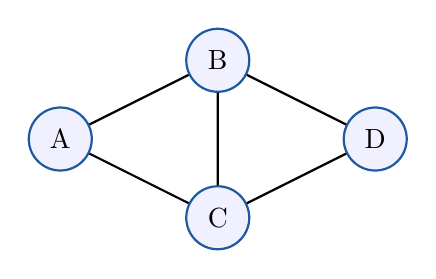
\begin{tikzpicture}[every node/.style={circle,draw=mathblue,fill=blue!6,minimum size=8mm},thick]\node(A) at (0,0){A};\node(B) at (2,1){B};\node(C) at (2,-1){C};\node(D) at (4,0){D};\draw(A)--(B)(A)--(C)(B)--(C)(B)--(D)(C)--(D);\end{tikzpicture}\end{center}
\section{Degree and paths}
The degree of a node is the number of edges touching it. In the diagram above, $\deg(A)=2$ and $\deg(B)=3$. A path is a sequence of nodes joined by edges. For example, $A\to B\to D$ is a path of length 2 (two edges). A shortest path uses as few edges as possible.
\textbf{Example.} If a message can travel along each edge in one round, then after one round from A it can reach B and C. After two rounds it may also reach D. A node with many immediate neighbors can spread a message quickly, though degree alone does not tell the whole story.
\section{Connected components and bottlenecks}
A network is connected if a path joins every pair of nodes. If not, it consists of separate connected components. An edge is a bridge if removing it disconnects part of the network. Bridges matter in roads, supply chains, communication, and social contact: a low-degree link can be structurally important even when its endpoints have few connections.
\section{Diffusion and collective behavior}
Diffusion describes how something moves through links: information, a behavior, a resource, or (in a simplified model) an infection. A basic discrete model starts with a set of active nodes. At each step, activity may pass to neighboring nodes. The model's assumptions matter: transmission may not be certain, connections may be directed, and people may respond differently.
\section{Networks and feedback}
A network describes who or what can influence whom. Feedback describes how a system responds to measured outcomes. Together they help explain collective systems: a change at one node can spread along paths, alter other nodes, and feed back into later decisions. A network diagram does not predict behavior by itself; it makes structure visible so that questions about reach, resilience, and bottlenecks can be asked clearly.
\section{A practical workflow}
\begin{enumerate}[label=\arabic*.]\item Name the nodes and define what an edge means.\item List or draw the edges.\item Use degree to count direct connections and paths to trace reach.\item Check connectedness and look for bridges or bottlenecks.\item State what the model leaves out, such as link strength, direction, time, or uncertainty.\end{enumerate}
\section*{Practice}
\begin{enumerate}\item For edges $AB, AC, AD, BE, CE$, find the degree of A and E.\item Is there a path from D to E? Give one if it exists.\item If A starts a one-step spread, how many new nodes are reached?\item In the path $A-B-C-D$, which edge is a bridge?\item Give one limitation of using an unweighted graph to model a real social network.\end{enumerate}
\section*{Key ideas}\begin{itemize}\item $G=(V,E)$ records nodes and links.\item Degree counts immediate neighbors; path length counts edges.\item Connectedness asks whether paths join every pair.\item Diffusion follows connections over time.\item Network structure can reveal bottlenecks without fully predicting behavior.\end{itemize}
\end{document}
% Build the companion course PDF from this source.
